\documentclass[12pt,a4paper]{article}
\usepackage{ctex}
\usepackage{amsmath,amssymb,bm}
\usepackage{geometry}
\usepackage{graphicx}
\geometry{left=2.5cm,right=2.5cm,top=2.5cm,bottom=2.5cm}

\title{CAGD 作业 6 实验报告}
\author{15 刘行}
\date{\today}

\begin{document}

\maketitle

\tableofcontents
\newpage

% ==========================================================
\section{题目 1:三次多项式曲线 \(P(u)\)(区间 [2,4])}

\subsection{题设}
\[
P(u)=
A\,u^3+B\,u^2+C\,u+D,\quad
\begin{aligned}
A&=-\begin{pmatrix}\tfrac78\\[2pt]\tfrac58\end{pmatrix},&
B&=\begin{pmatrix}9\\[2pt]\tfrac{15}{4}\end{pmatrix},\\[4pt]
C&=-\begin{pmatrix}\tfrac{57}{2}\\[2pt]\tfrac{9}{2}\end{pmatrix},&
D&=\begin{pmatrix}30\\[2pt]-1\end{pmatrix}.
\end{aligned}
\]

\subsection{(1) 极坐标形式与 Bézier 控制点}

标量三次多项式的极坐标形式为:
\[
p[u_1,u_2,u_3]
=a\,u_1u_2u_3+\frac{b}{3}(u_1u_2+u_1u_3+u_2u_3)+\frac{c}{3}(u_1+u_2+u_3)+d.
\]

因此向量形式为:
\[
\boxed{
P[u_1,u_2,u_3]
=A\,u_1u_2u_3+\tfrac13 B\!\sum_{\text{sym}} u_i u_j+\tfrac13 C(u_1+u_2+u_3)+D.
}
\]

将区间 \([2,4]\) 线性重参到 \(t\in[0,1]\):  
\[
t=\frac{u-2}{2}.
\]

三次多项式在任意区间 \([a,b]\) 上的 Bézier 控制点满足:
\[
\boxed{
\begin{aligned}
P_0&=P(a),&
P_1&=P(a)+\frac{b-a}{3}P'(a),\\
P_2&=P(b)-\frac{b-a}{3}P'(b),&
P_3&=P(b).
\end{aligned}}
\]

其中 \(a=2,\ b=4,\ \frac{b-a}{3}=\frac{2}{3}\)。  
一阶导数为:
\[
P'(u)=3A\,u^2+2B\,u+C.
\]
计算得:
\[
\begin{aligned}
P(2)&=(2,0), & P'(2)&=(-3,3);\\
P(4)&=(4,1), & P'(4)&=\left(\tfrac32,-\tfrac{9}{2}\right).
\end{aligned}
\]
因此:
\[
\boxed{
\begin{aligned}
P_0&=(2,0),\\
P_1&=(0,2),\\
P_2&=(3,4),\\
P_3&=(4,1).
\end{aligned}}
\]

控制多边形为 \((2,0)\to(0,2)\to(3,4)\to(4,1)\)。

\subsection{(2) 用 de Casteljau 算法求值}

参数转换 \(t=(u-2)/2\),当 \(u=\{2.5,3,3.5\}\) 时,\(t=\{1/4,1/2,3/4\}\)。  
以控制点 \(P_0=(2,0),P_1=(0,2),P_2=(3,4),P_3=(4,1)\) 运算。

\paragraph{计算结果:}

\begin{itemize}
\item \(t=\tfrac14(u=2.5)\):
  \(\boxed{(\tfrac{85}{64},\tfrac{91}{64})}\)
\item \(t=\tfrac12(u=3)\):
  \(\boxed{(\tfrac{15}{8},\tfrac{19}{8})}\)
\item \(t=\tfrac34(u=3.5)\):
  \(\boxed{(\tfrac{191}{64},\tfrac{153}{64})}\)
\end{itemize}

\paragraph{代码实现:}
见 \texttt{src/main\_1.m}

\paragraph{程序输出:}
\begin{verbatim}
Sample points [x y] at u={2.5,3,3.5}:
    1.3281    1.4219
    1.8750    2.3750
    2.9844    2.3906
\end{verbatim}

\paragraph{结果图像:}
\begin{center}
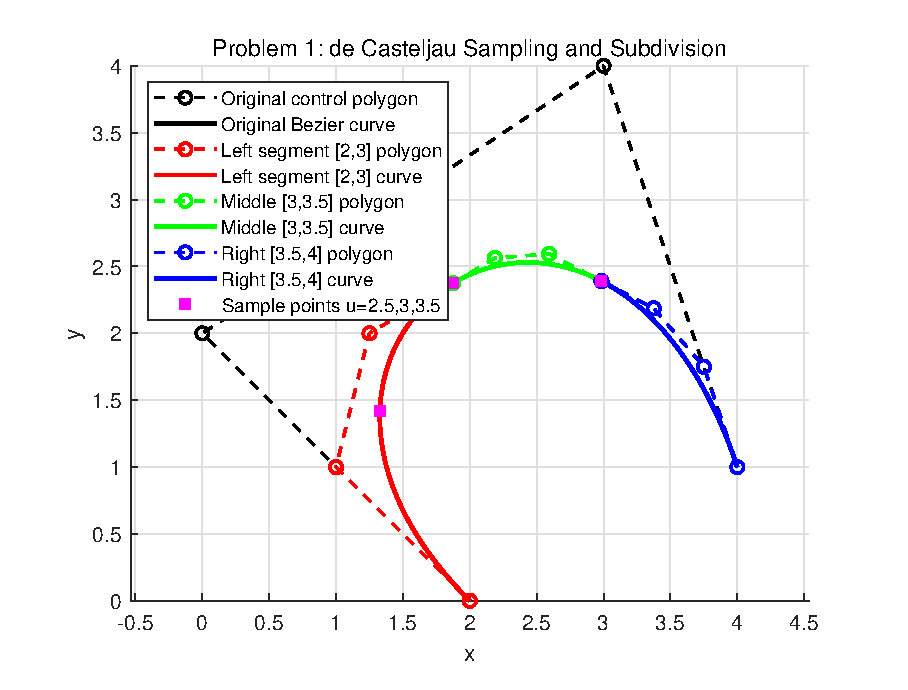
\includegraphics[width=0.8\textwidth]{fig/problem1.eps}
\end{center}

\subsection{(3) 曲线分割}

在 \(u=3\) 处分割,得到左右两段 Bézier 曲线;再将右半段在 \(u=3.5\) 处分割,得到三段曲线。

\begin{itemize}
\item 左段控制点:\((2,0),(1,1),(\tfrac54,2),(\tfrac{15}{8},\tfrac{19}{8})\)
\item 中段控制点:\((\tfrac{15}{8},\tfrac{19}{8}),(\tfrac{35}{16},\tfrac{41}{16}),(\tfrac{83}{32},\tfrac{83}{32}),(\tfrac{191}{64},\tfrac{153}{64})\)
\item 右段控制点:\((\tfrac{191}{64},\tfrac{153}{64}),(\tfrac{27}{8},\tfrac{35}{16}),(\tfrac{15}{4},\tfrac{7}{4}),(4,1)\)
\end{itemize}

最终绘制出三条子控制多边形与对应曲线(见上图)。

% ==========================================================
\section{题目 2:三次多项式曲线 \(F(u)\)(区间 [0,1])}

\[
F(u)=
\begin{pmatrix}
15\\[-2pt]-6
\end{pmatrix}u^3+
\begin{pmatrix}
27\\[-2pt]10
\end{pmatrix}u^2-
\begin{pmatrix}
9\\[-2pt]9
\end{pmatrix}u.
\]

\subsection{(1) 一、二阶导数}
\[
\boxed{
\begin{aligned}
F'(u)&=
\begin{pmatrix}
45\\[-2pt]-18
\end{pmatrix}u^2+
\begin{pmatrix}
54\\[-2pt]20
\end{pmatrix}u-
\begin{pmatrix}
9\\[-2pt]9
\end{pmatrix},\\[4pt]
F''(u)&=
\begin{pmatrix}
90\\[-2pt]-36
\end{pmatrix}u+
\begin{pmatrix}
54\\[-2pt]20
\end{pmatrix}.
\end{aligned}}
\]

\subsection{(2) 极坐标形式与恒等式证明}

设
\[
F[u_1,u_2,u_3]
=A\,u_1u_2u_3+\tfrac{B}{3}\sum_{\text{sym}}u_iu_j+\tfrac{C}{3}(u_1+u_2+u_3)+D.
\]

则
\[
f(u_1,u_2,\hat{1})
=f(u_1,u_2,1)-f(u_1,u_2,0)
=A\,u_1u_2+\frac{B}{3}(u_1+u_2)+\frac{C}{3}.
\]
因此:
\[
\boxed{3f(u_1,u_2,\hat{1})=3A\,u_1u_2+B(u_1+u_2)+C,}
\]
这正是 \(F'(u)=3A\,u^2+2B\,u+C\) 的极坐标形式。

再求二阶差分:
\[
f(u_1,\hat{1},\hat{1})=A\,u_1+\tfrac{B}{3},\quad
6f(u_1,\hat{1},\hat{1})=6A\,u_1+2B,
\]
正好对应 \(F''(u)=6A\,u+2B\)。证毕。

% ==========================================================
\section{题目 3:均匀 B 样条(节点向量 [0,0,1,2,3,4,5,5])}

控制点:
\[
P_0=(-2,-10),\quad P_1=(-4,2),\quad P_2=(6,5),\quad P_3=(4,-7).
\]

\subsection{(1) 用 de Boor 算法计算 \(t=2.5\) 处的位置}

在 \([2,3)\) 区间内(\(k=3\)):
\[
\begin{aligned}
r=1: &\ (-\tfrac{11}{3},0),(1,\tfrac72),(\tfrac{17}{3},3),\\
r=2: &\ (-\tfrac{1}{6},\tfrac{21}{8}),(\tfrac{13}{6},\tfrac{27}{8}),\\
r=3: &\ \boxed{C(2.5)=(1,3)}.
\end{aligned}
\]
该点由程序验证。

\paragraph{程序代码:}
见 \texttt{src/main\_3.m}

\paragraph{程序输出:}
\begin{verbatim}
Curve point at t = 2.5:
     1     3

Equivalent cubic Bezier control points [x y]:
   -2.0000    0.5000
   -0.6667    3.0000
    2.6667    4.0000
    4.0000    2.5000
\end{verbatim}

\paragraph{结果图像:}
\begin{center}
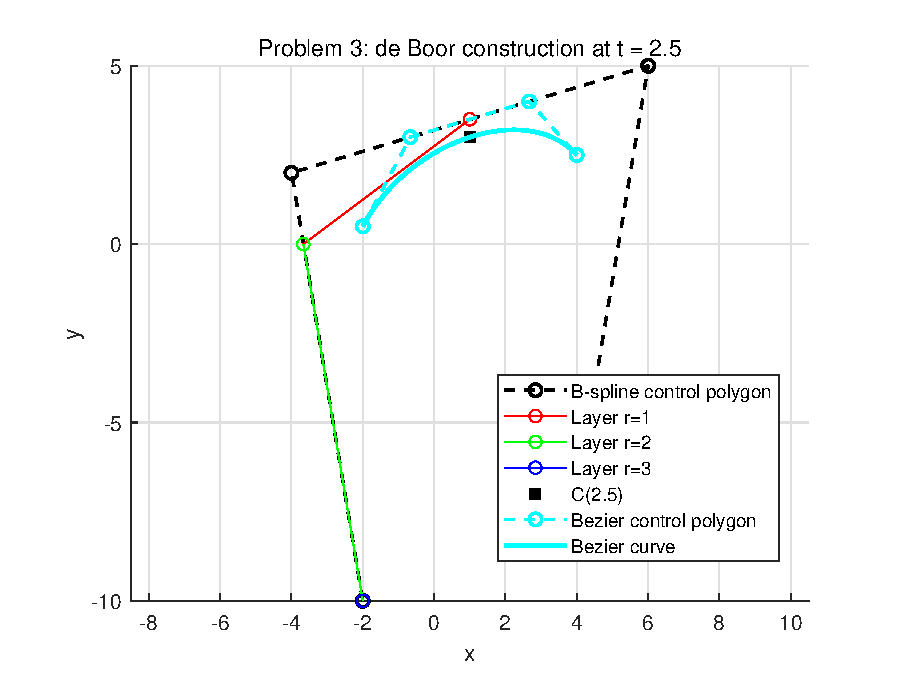
\includegraphics[width=0.8\textwidth]{fig/problem3.eps}
\end{center}

\subsection{(2) 转换为 Bézier 形式}

根据端点与导数:
\[
\boxed{
\begin{aligned}
B_0&=C(2),&
B_1&=C(2)+\frac{1}{3}C'(2),\\
B_2&=C(3)-\frac{1}{3}C'(3),&
B_3&=C(3).
\end{aligned}}
\]

代入计算:
\[
B_0=(-2,0.5),\quad
B_1=(-\tfrac{2}{3},3),\quad
B_2=(\tfrac{8}{3},4),\quad
B_3=(4,2.5).
\]

在该 Bézier 曲线取 \(t=0.5\) 得 \((1,3)\),与 B 样条计算一致。

\end{document}
